% Set Title, Author, and email
\title{ELE0646 - Chaves fusíveis}
\author{Levy Gabriel da S. G. \\ Engenharia elétrica - UFRN}

\maketitle
\thispagestyle{fancy}

\begin{itemize}
    \item Sobrecarga: não é considerado um defeito, com correntes de 10x a nominal;
    \item Curto-circuito: defeito, ocorrendo quando a impedância entre dois pontos é reduzida a valores próximos de zero, com intensidade maior que 10x a corrente nominal;
\end{itemize}

\textbf{Aplicações}

\begin{itemize}
    \item Proteção de TRAFOs de força de SEs de concessionária e by-pass de disjuntores/religadores de circuitos de distribuição de MT;
    \item Montagem nas estruturas de subestações;
    \item Constituídas por dois isoladores em uma base metálica;
\end{itemize}

\textbf{Partes constituintes}

\begin{itemize}
    \item Isolador;
    \item Suporte de fixação;
    \item Cartucho, porta-fusível ou "canela";
    \item Terminal de fonte;
    \item Terminal de carga;
    \item Articulação;
    \item Elo fusível (dentro do cartucho).
    \begin{itemize}
        \item Tipos:
        \begin{itemize}
            \item Botão;
            \item Argola ou olhal.
        \end{itemize}
        \item Partes:
        \begin{itemize}
            \item Elemento fusível;
            \item Tubinho;
            \item Rabicho.
        \end{itemize}
    \end{itemize}
\end{itemize}

\textbf{Curvas de atuação}

\begin{itemize}
    \item Curva dos tempos mínimos de fusão: curva mais baixa de cada elo (vermelho);
    \item Curva dos máximos tempos de interrupção: curva mais alta de cada elo (preto);
    \item O tempo de arco é a diferença de tempo entre as duas curvas;
\end{itemize}

\textbf{Tipos de ele fusível}

\begin{itemize}
    \item Elos fusíveis de distribuição:
    \begin{itemize}
        \item Elo tipo H (alto surto);
        \begin{itemize}
            \item Ação lenta, fabricado para pequenas correntes nominais, para proteção de TRAFOS de até 75kVA e bancos de capacitores;
            \item Elos da série H: 1H, 2H, 3H e 5H;
            \item Elos da série H não possuem capacidade de sobrecarga e começam a operar a partir de 1.5 vezes a sua corrente nominal num tempo de 300s.
        \end{itemize}
        \item Elo tipo K (elos rápidos);
        \item Elo tipo T (elos lentos).
        \begin{itemize}
            \item Os elos do tipo K e T são empregados na proteção de ramais de circuitos de distribuição de MT e proteção contra sobrecorrentes para TRAFOS entre 112.5kVA e 300kVA (acima desse valor a proteção deve ser realizada por disjuntores com relés);
            \item Para elos fusíveis de mesma corrente nominal, os elos da família K são mais rápidos do que os da família T, sendo assim mais utilizados;
            \item Classes da família K:
            \begin{itemize}
                \item Elos preferenciais: 6K, 10K, 15K, 25K, 40K, 65K, 100K, 140K e 200K;
                \item Elos não-preferenciais: 8K, 12K, 20K, 30K, 50K e 80K. 
            \end{itemize}
            \item Os elos K e T admitem sobrecargas de até 1.5 vezes as suas correntes nominais sem causar excesso de temperatura à chave-fusível;
            \item A fusão dos elos K e T ocorrem em aproximadamente 2 vezes os seus valores nominais em um tempo de 300 segundos.
        \end{itemize}
    \end{itemize}
   \item Elos fusíveis de força:
   \begin{itemize}
        \item Elo tipo EF (elos rápidos);
        \item Elo tipo ES (elos lentos).
    \end{itemize}
\end{itemize}

\textbf{Coordenação entre elos fusíveis}

\begin{itemize}
    \item O sistema será coordenado quando efeitos a jusante do elo fusível protetor não provocarem o desligamento do elo fusível protegido:
    \begin{itemize}
        \item Elemento protetor é aquele mais próximo ao defeito;
        \item Elemento protegido é a proteção de retaguarda, mais distante do ponto de defeito.
    \end{itemize}
    \item O elo protetor deve atuar primeiro que o protegido;
    \item Os elos fusíveis adjacentes das séries preferencial e não preferencial não apresentam coordenação (elo protetor 6K[preferencial] não coordenada com elo protegido de 8K[não preferencial], mas coordena com elo de 10K[preferencial] e 12K[não preferencial]);
    \item Geralmente utiliza-se a série preferencial por possuírem mais opções, assim aumentando flexibilidade.
\end{itemize}

\textbf{Especificação das chaves-fusíveis}

\begin{itemize}
    \item Tensão nominal;
    \item NBI;
    \item Corrente nominal;
    \item Capacidade de ruptura ou corrente de interrupção.
\end{itemize}

\textbf{Dimensionamento da chave-fusível}
\begin{itemize}
    \item A corrente do cartucho da chave-fusível deve ser igual ou superior à corrente admissível do fusível multiplicada por um fator K: $|I_{NOM}^{CF}| > K \times |I_{ADM}^{FS}|$
    \item A corrente de interrupção da chave-fusível deve ser igual ou superior ao valor assimétrico da corrente de curto-circuito no ponto de instalação da chave: $|I_{INT}^{CF}| \leq |I_{CC}^{ASM}|$
\end{itemize}

\textbf{Dimensionamento do elo-fusível}
\begin{itemize}
    \item Operar para curtos-circuitos no TRAFO e na rede secundária;
    \item Não confundir a sobrecarga permissível no TRAFO (para TRAFOS de distribuição admite-se sobrecarga de até $2 \times I_{NTRAFO}$ durante um tempo de 0.1s (6 ciclos de 60Hz));
    \item Não confundir a corrente de \textit{inrush}, estimada em $8 \text{ou} 12 \times I_{NTRAFO}$, durante um tempo de 0.1s (6 ciclos de 60Hz);
    \item Deve coordenar as proteções a montante;
    \item A curva de interrupção do elo deverá estar abaixo da curva térmica do TRAFO.
    \begin{table}[H]
\centering
\begin{tabular}{|c|c|c|}
\hline
Potência do transformador (kVA) & Corrente (A) & Fusível (A) \\ \hline
15                              & 0.63         & 1H          \\ \hline
30                              & 1.26         & 2H          \\ \hline
45                              & 1.88         & 3H          \\ \hline
75                              & 3.14         & 5H          \\ \hline
112.5                           & 4.71         & 6K          \\ \hline
150                             & 6.28         & 8K          \\ \hline
225                             & 9.41         & 10K         \\ \hline
300                             & 12.55        & 15K         \\ \hline
\end{tabular}
\end{table}
\end{itemize}


\begin{figure}[H]
\begin{center}
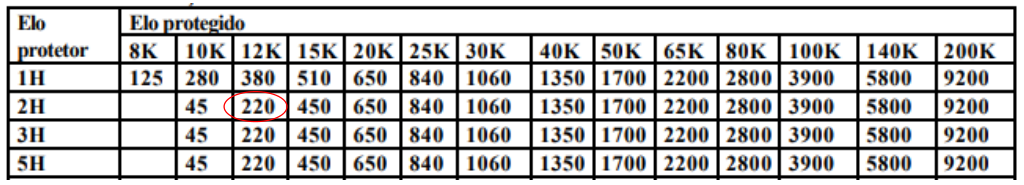
\includegraphics[width=16cm]{tabela1.PNG}  
\label{fig:1} 
\end{center}
\end{figure}

\begin{figure}[H]
\begin{center}
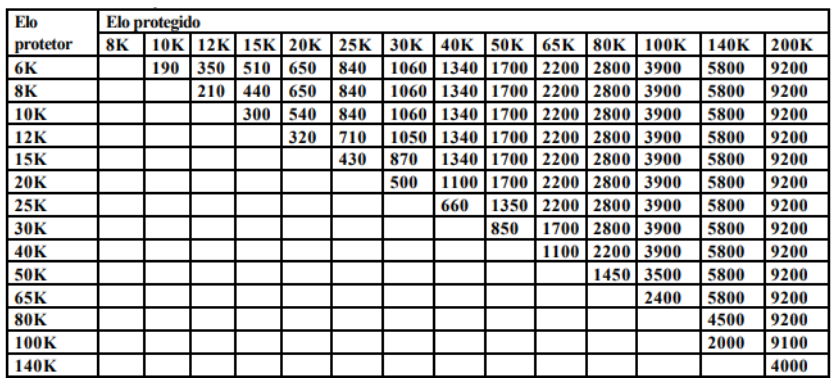
\includegraphics[width=16cm]{tabela2.PNG}  
\label{fig:2} 
\end{center}
\end{figure}

\begin{figure}[H]
\begin{center}
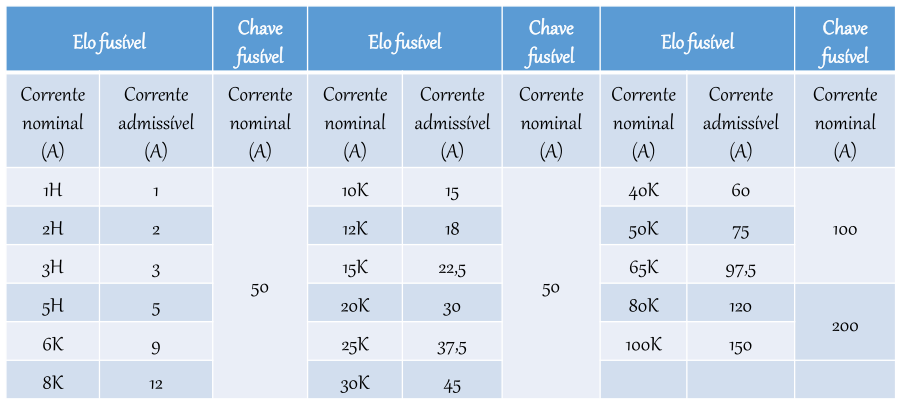
\includegraphics[width=16cm]{tabela3.PNG}  
\label{fig:3} 
\end{center}
\end{figure}

\begin{figure}[H]
\begin{center}
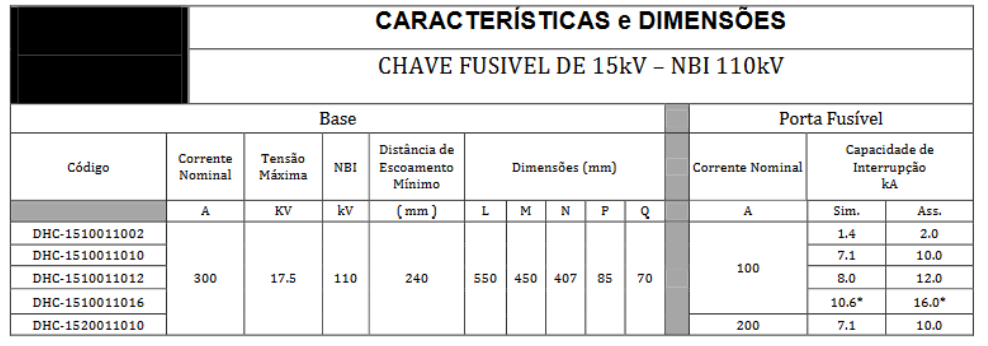
\includegraphics[width=16cm]{tabela4.PNG}  
\label{fig:4} 
\end{center}
\end{figure}